%############################################# ANDRÁS KISS ##########################################
%################################################ 2018 ##############################################
\documentclass[a4paper, 11pt, oneside, bibliography=totoc]{article}
%\def\magyarOptions{hyphenation=huhyphn}
\usepackage{ae,aecompl}
\usepackage[T1]{fontenc}
\usepackage[utf8]{inputenc}
%\usepackage[hungarian]{babel}
\usepackage{indentfirst}
\usepackage{xymtex}
\usepackage{multirow}
\usepackage{gensymb}
\usepackage{upgreek}
\usepackage[geometry]{ifsym}
\usepackage{subfig}
\usepackage[version=3]{mhchem}
\usepackage{float}
\usepackage{textcomp}
\frenchspacing
\usepackage[dvips]{graphicx}
\usepackage{color}
\usepackage{anysize}
\marginsize{3.2cm}{2.8cm}{3cm}{2cm}
\usepackage{enumerate}
\usepackage{cite}
\usepackage{listings}
\usepackage{setspace}
\usepackage{marginnote}
\setstretch{1.2}
\usepackage{xcolor}
\usepackage{listings}
\usepackage[font={small}]{caption}

\definecolor{codegreen}{rgb}{0,0.6,0}
\definecolor{codegray}{rgb}{0.5,0.5,0.5}
\definecolor{codepurple}{rgb}{0.58,0,0.82}
\definecolor{backcolour}{rgb}{0.95,0.95,0.92}
\lstdefinestyle{mystyle}{
    backgroundcolor=\color{backcolour},   
    commentstyle=\color{codegreen},
    keywordstyle=\color{magenta},
    numberstyle=\tiny\color{codegray},
    stringstyle=\color{codepurple},
    basicstyle=\footnotesize,
    breakatwhitespace=false,         
    breaklines=true,                 
    captionpos=b,                    
    keepspaces=true,                 
    numbers=left,                    
    numbersep=5pt,                  
    showspaces=false,                
    showstringspaces=false,
    showtabs=false,                  
    tabsize=2
}
\lstset{style=mystyle}


\begin{document}
\title{\emph{DAAD Scholarship} report}
\author{Dr. András Kiss}
\maketitle

In this document I summarize the most important results of the work I have done in the laboratory of prof. Markus Hoth at the Center of Integrative Physiology and Molecular Medicine (CIPMM) in Homburg during the time period of 11th June 2018 -- 10th of August 2018 under the supervision of Dr. Monika Bozem. The work was financially supported by the German Academic Exchange Service (Deutscher Akademischer Austausch Dienst, DAAD).

The main goal of the work was to map the H$_2$O$_2$ production of certain immune cells with the Scanning Electrochemical Microscope (SECM). Additionally, new protocols had to be worked out in order to accomplish that goal. 
%Among others, these include:

%\begin{itemize}
%\item production of 10 $\upmu$m or smaller diameter platinum microelectrodes,
%\item calibration and characterization of these,
%\end{itemize}

By the time I joined the electrochemistry team at CIPMM, a lot of successful work has already been done that is published in \cite{bozem2018electrochemical}. Upon my arrival, Dr. Bozem presented three recently discovered problems which had to be solved before electroactive species like H$_2$O$_2$ and O$_2$ could be mapped in the close vicinity of the immune cells by the SECM:
 
\begin{itemize}
\item high distortion in the images,
\item large amount of noise when the temperature is increased to the physiological 37 $\celsius$,
\item insufficient resolution of the cells due to the relatively large diameter of the platinum microelectrodes.
\end{itemize}

We selected the first one to be worked on. The reason for this is that I have experience with reconstructing SECM images by removing distortion based on theoretical models. The problem is shown in Fig. \ref{fig:deconv}B. When a monocyte (Fig. \ref{fig:deconv}A) is scanned with the SECM, the resulting image is distorted. Eventually I solved the problem with deconvolution (Fig. \ref{fig:deconv}C). With this improvement, H$_2$O$_2$ and othe electroactive species can be mapped with higher temporal resolution. This summary is mostly about how I did it. I managed to improve distorted H$_2$O$_2$ images recorded earlier by Dr. Monika Bozem and Phillip Knapp, and conducted my own experiments and applied the deconvolution on those as well. To investigate the problem, first I have reduced the complexity by creating a model system. It featured an ,,ideal'' step, that has a well defined geometry. The system consisted of a broken glass sheet in a Petri--dish. The broken edge of the glass sheet is very sharp, and creates a good step function. When the Pt UME is scanned above it, the measured current is low when the tip is close to the glass sheet, but once it reaches the edge and it is suddenly in the bulk of the solution, the current increases, because diffusion of the electroactive species (ferrocene) is no longer hindered. This is an ideal setup to study how the image of a near perfect step function is distorted by the scanning process. A sketch of the model system can be seen in Fig. \ref{fig:step}.

\begin{figure}
\centering
% trim = top left bottom right
% trim = left bottom right top
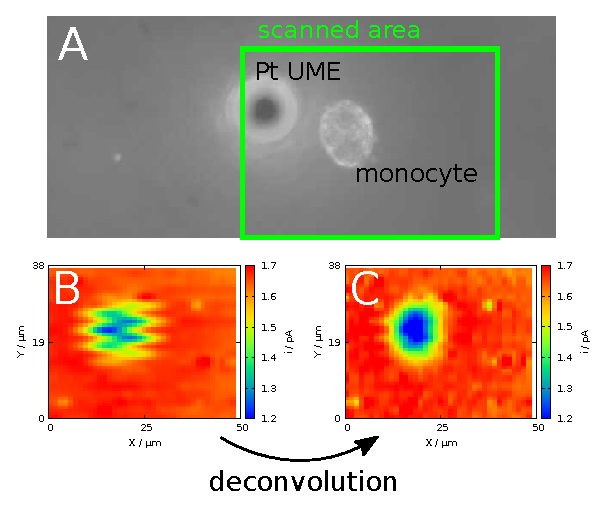
\includegraphics[width=0.8\textwidth]{deconv.eps}
\caption{(A) Optical microphoto of the setup including the monocyte, the platinum microelectrode tip and the scanned area. (B) Raw measurement. Values represent the tip current oxidizing H$_2$O$_2$ at the platinum tip. The distortion is visible along the alternating scanlines. (C) Deconvoluted image obtained from (B).}
\label{fig:deconv}
\end{figure} 


The result of the SECM scanning is presented in Fig. \ref{fig:step}B. When the system is scanned with a speed of 5 $\upmu$m/s, the image is not distorted. However, when the speed was increased to 10 $\upmu$m/s, the image became distorted (Fig. \ref{fig:step}C). This speed is still insufficient to investigate a monocyte with fairly good temporal resolution. The distortion is very similar I have encountered during my PhD studies \cite{kiss2015deconvolution, kiss2015deconvolution2}. In that case, the distortion was caused by the relatively large RC time-constant ot he potentiometric cell. I could solve that by working out a deconvolution algorithm. In this case, the distortion is caused by slow amperometric response that is associated with the Cottrell--equation, but also with the RC time-constant. Therefore the transfer function describing the distortion includes at least two factors: $1/\sqrt{t}$ from the Cottrell--equation and $e^{-t/RC}$ from the time constant of the RC circuit element that is present in the amperometric cells as well as potentiometric cells. The deconvolution function is the inverse of those functions. I have written the following Python program to perform the deconvolution:

\begin{lstlisting}{language=python}
#!/usr/bin/enc python

# Here is a first attempt at porting the deconvolution algorithm
# from FORTRAN to python and applying it on amperometric SECM images.
# The gaussian filter is not yet implemented in the program.
# Right now I do it with the plotting software (gnuplot),
# but it would be better if the python program did it. Also, I haven't
# done the command line argument interpreter yet, so the file name must
# be changed in the code every time. A GUI would be nice, and a live plot
# of the convoluted and deconvoluted image. For that, the XYZ data needs
# to be converted to a matrix.

import numpy as np

conv_img = np.loadtxt("11.txt")
deconv_img = np.copy(conv_img)
e0 = np.float32(conv_img[0][2])
for n in range(0, conv_img.shape[0]):
 deconv_img[n][2] = np.float32((conv_img[n][2]-e0*0.985)/(1-0.985))
 e0 = np.float32(conv_img[n][2])

np.savetxt("11_python_deconvoluted.txt", deconv_img, delimiter=" ")
\end{lstlisting}

Quite surprisingly, after deconvolution, the image became even more distorted (Fig. \ref{fig:step}D). The explanation is the following. It is a well known fact from hydrodynamics, that when two planes close to each other move relatively to each other in a liquid, and when one reaches the edge of the other, a very strong convective effect is present. This is depicted in Fig. \ref{fig:step}E. This effect increases the current for a short time when the electrode is moving from above the glass sheet cover to the bulk. The change is more sudden than when it is moving in the opposite direction and it negates the delaying effect.

\begin{figure}
\centering
\begin{flushleft} \hspace{3cm}A\end{flushleft}

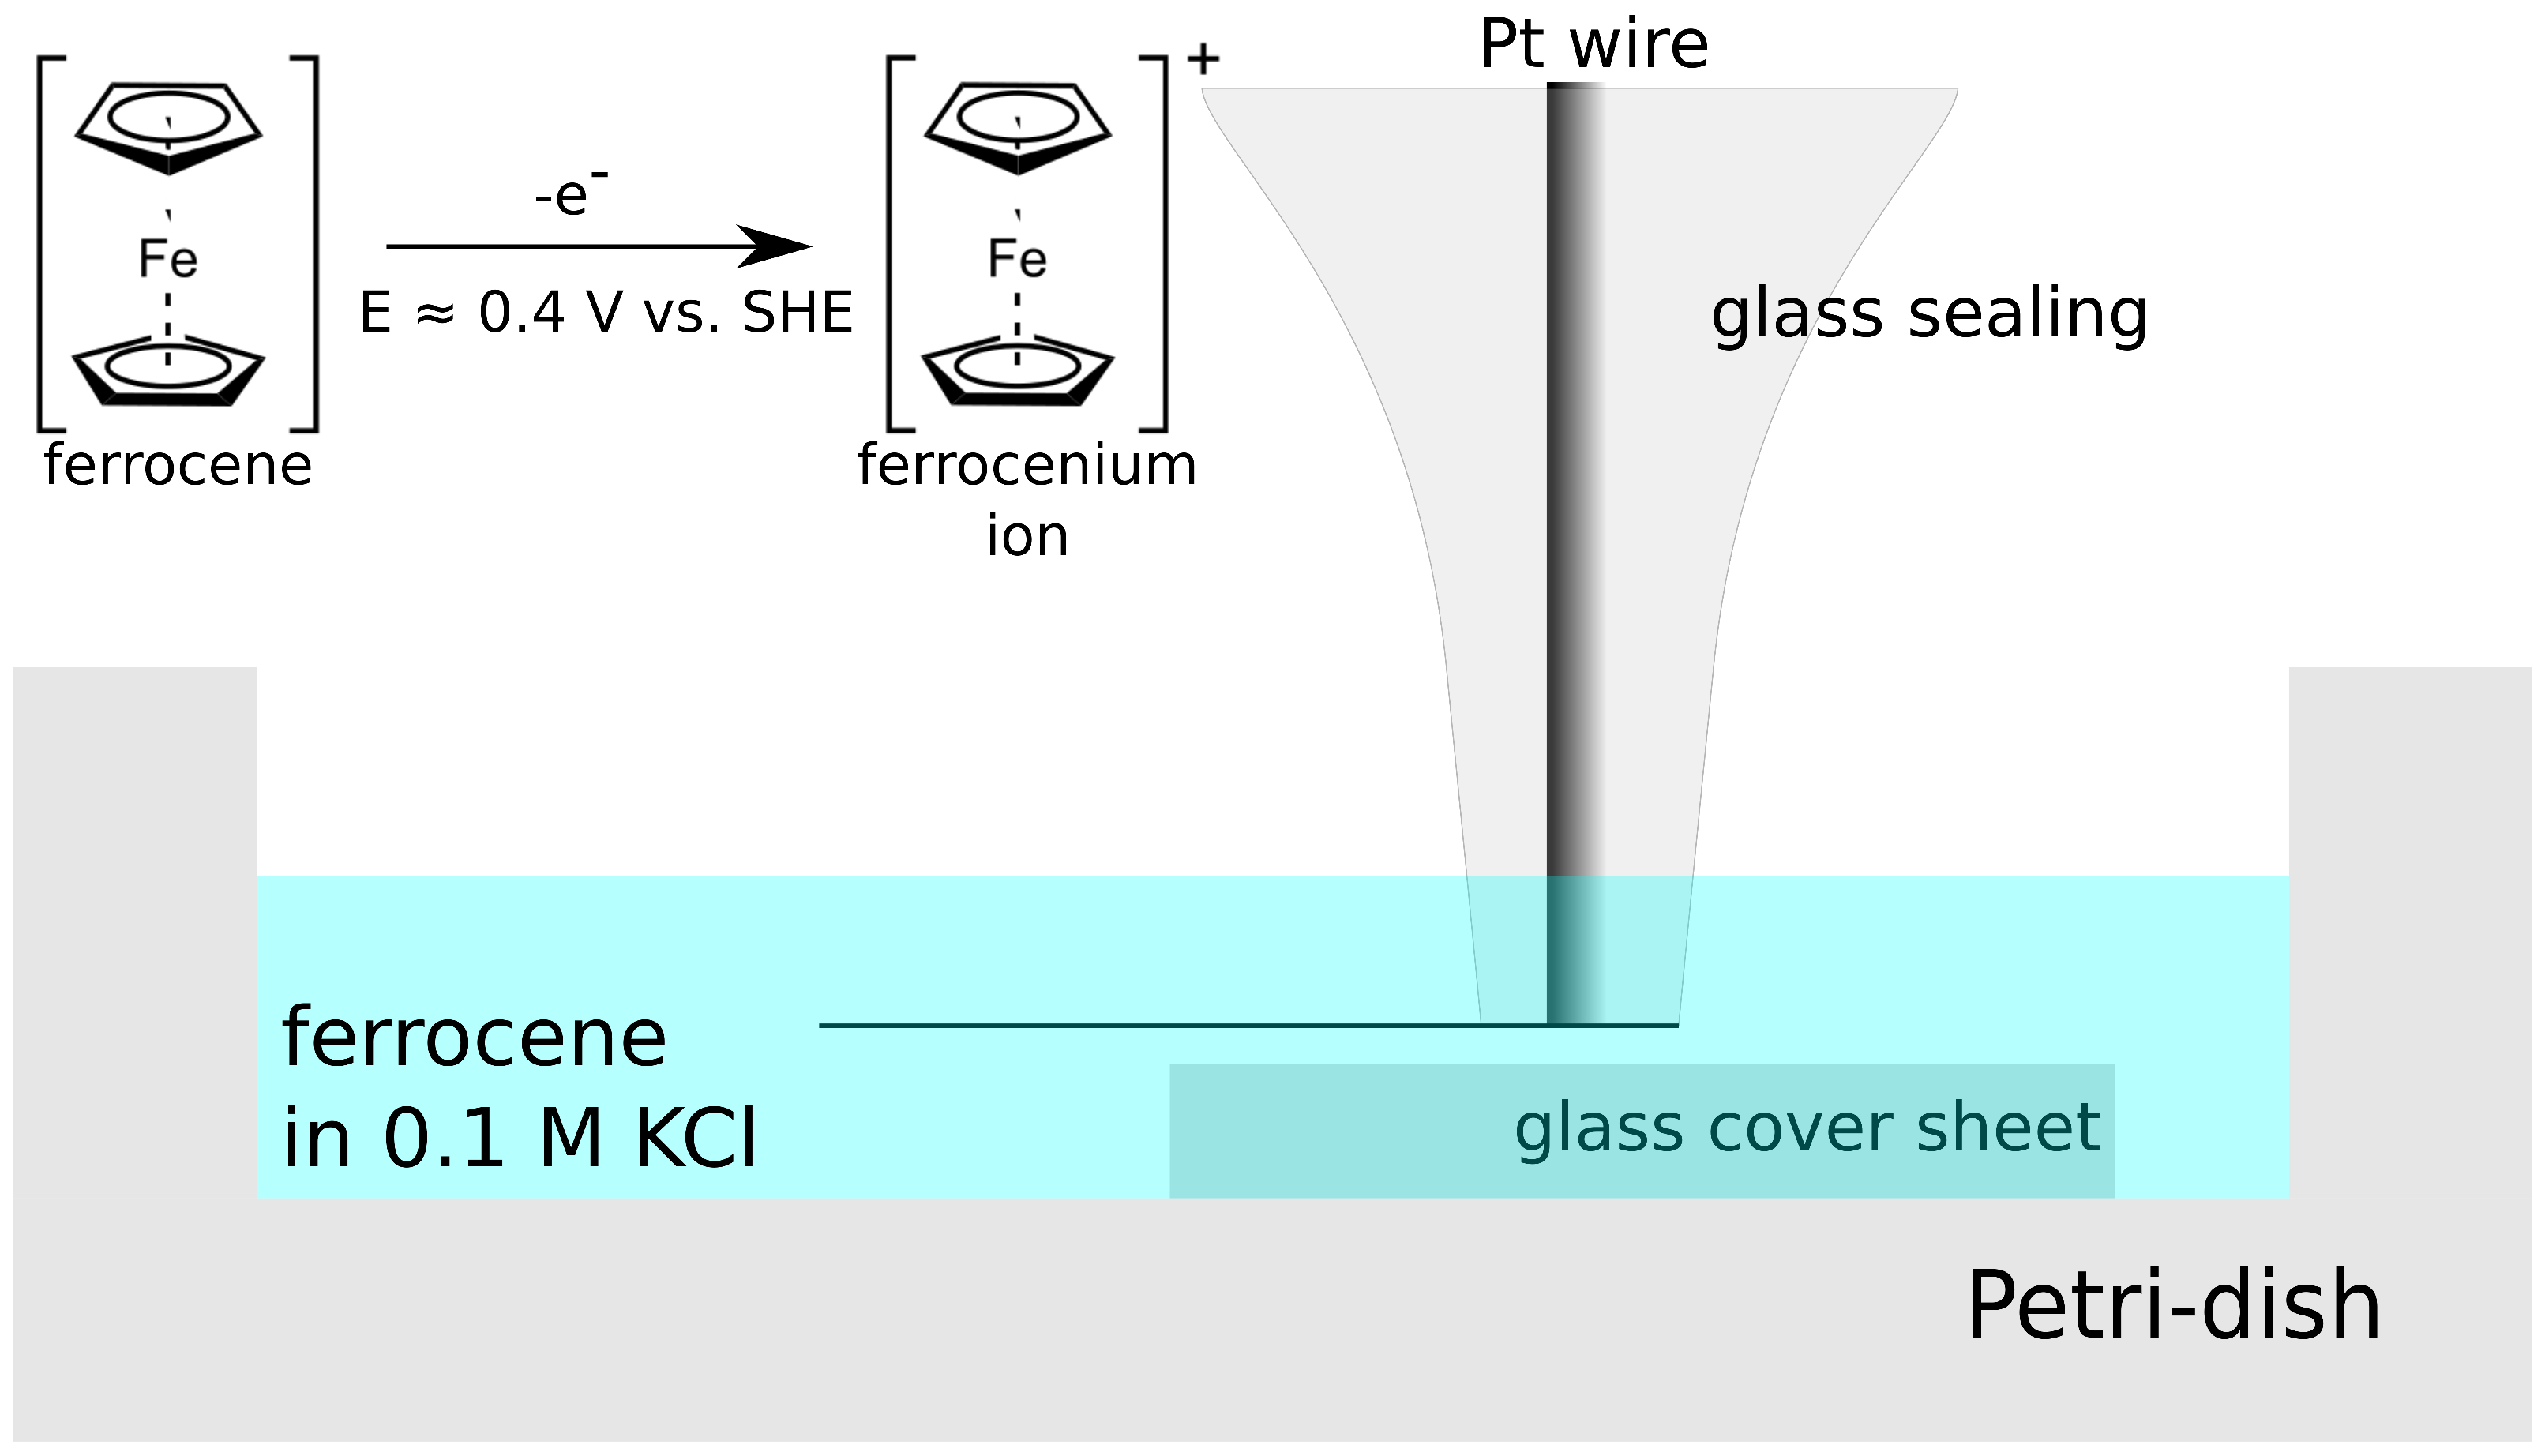
\includegraphics[width=0.5\textwidth]{step.eps}
\vspace{0.5cm}

\hspace{0.3cm} B \hspace{3.4cm} C \hspace{3.6cm} D \hfill
%\begin{flushleft}A\end{flushleft}

\includegraphics[trim = 10mm 60mm 0mm 60mm, clip, width=0.33\textwidth, angle=-90]{1.eps}\includegraphics[trim = 10mm 60mm 0mm 60mm, clip, width=0.33\textwidth, angle=-90]{2_meandered.eps}\includegraphics[trim = 10mm 60mm 0mm 60mm, clip, width=0.33\textwidth, angle=-90]{2_meandered_deconvoluted.eps}

\hspace{1.3cm} 5 $\upmu$m/s \hspace{2.5cm} 10 $\upmu$m/s \hspace{1.2cm} 10 $\upmu$m/s deconvoluted \hfill

\vspace{0.5cm}
\begin{flushleft}\hspace{3cm}E\end{flushleft}

\centering
 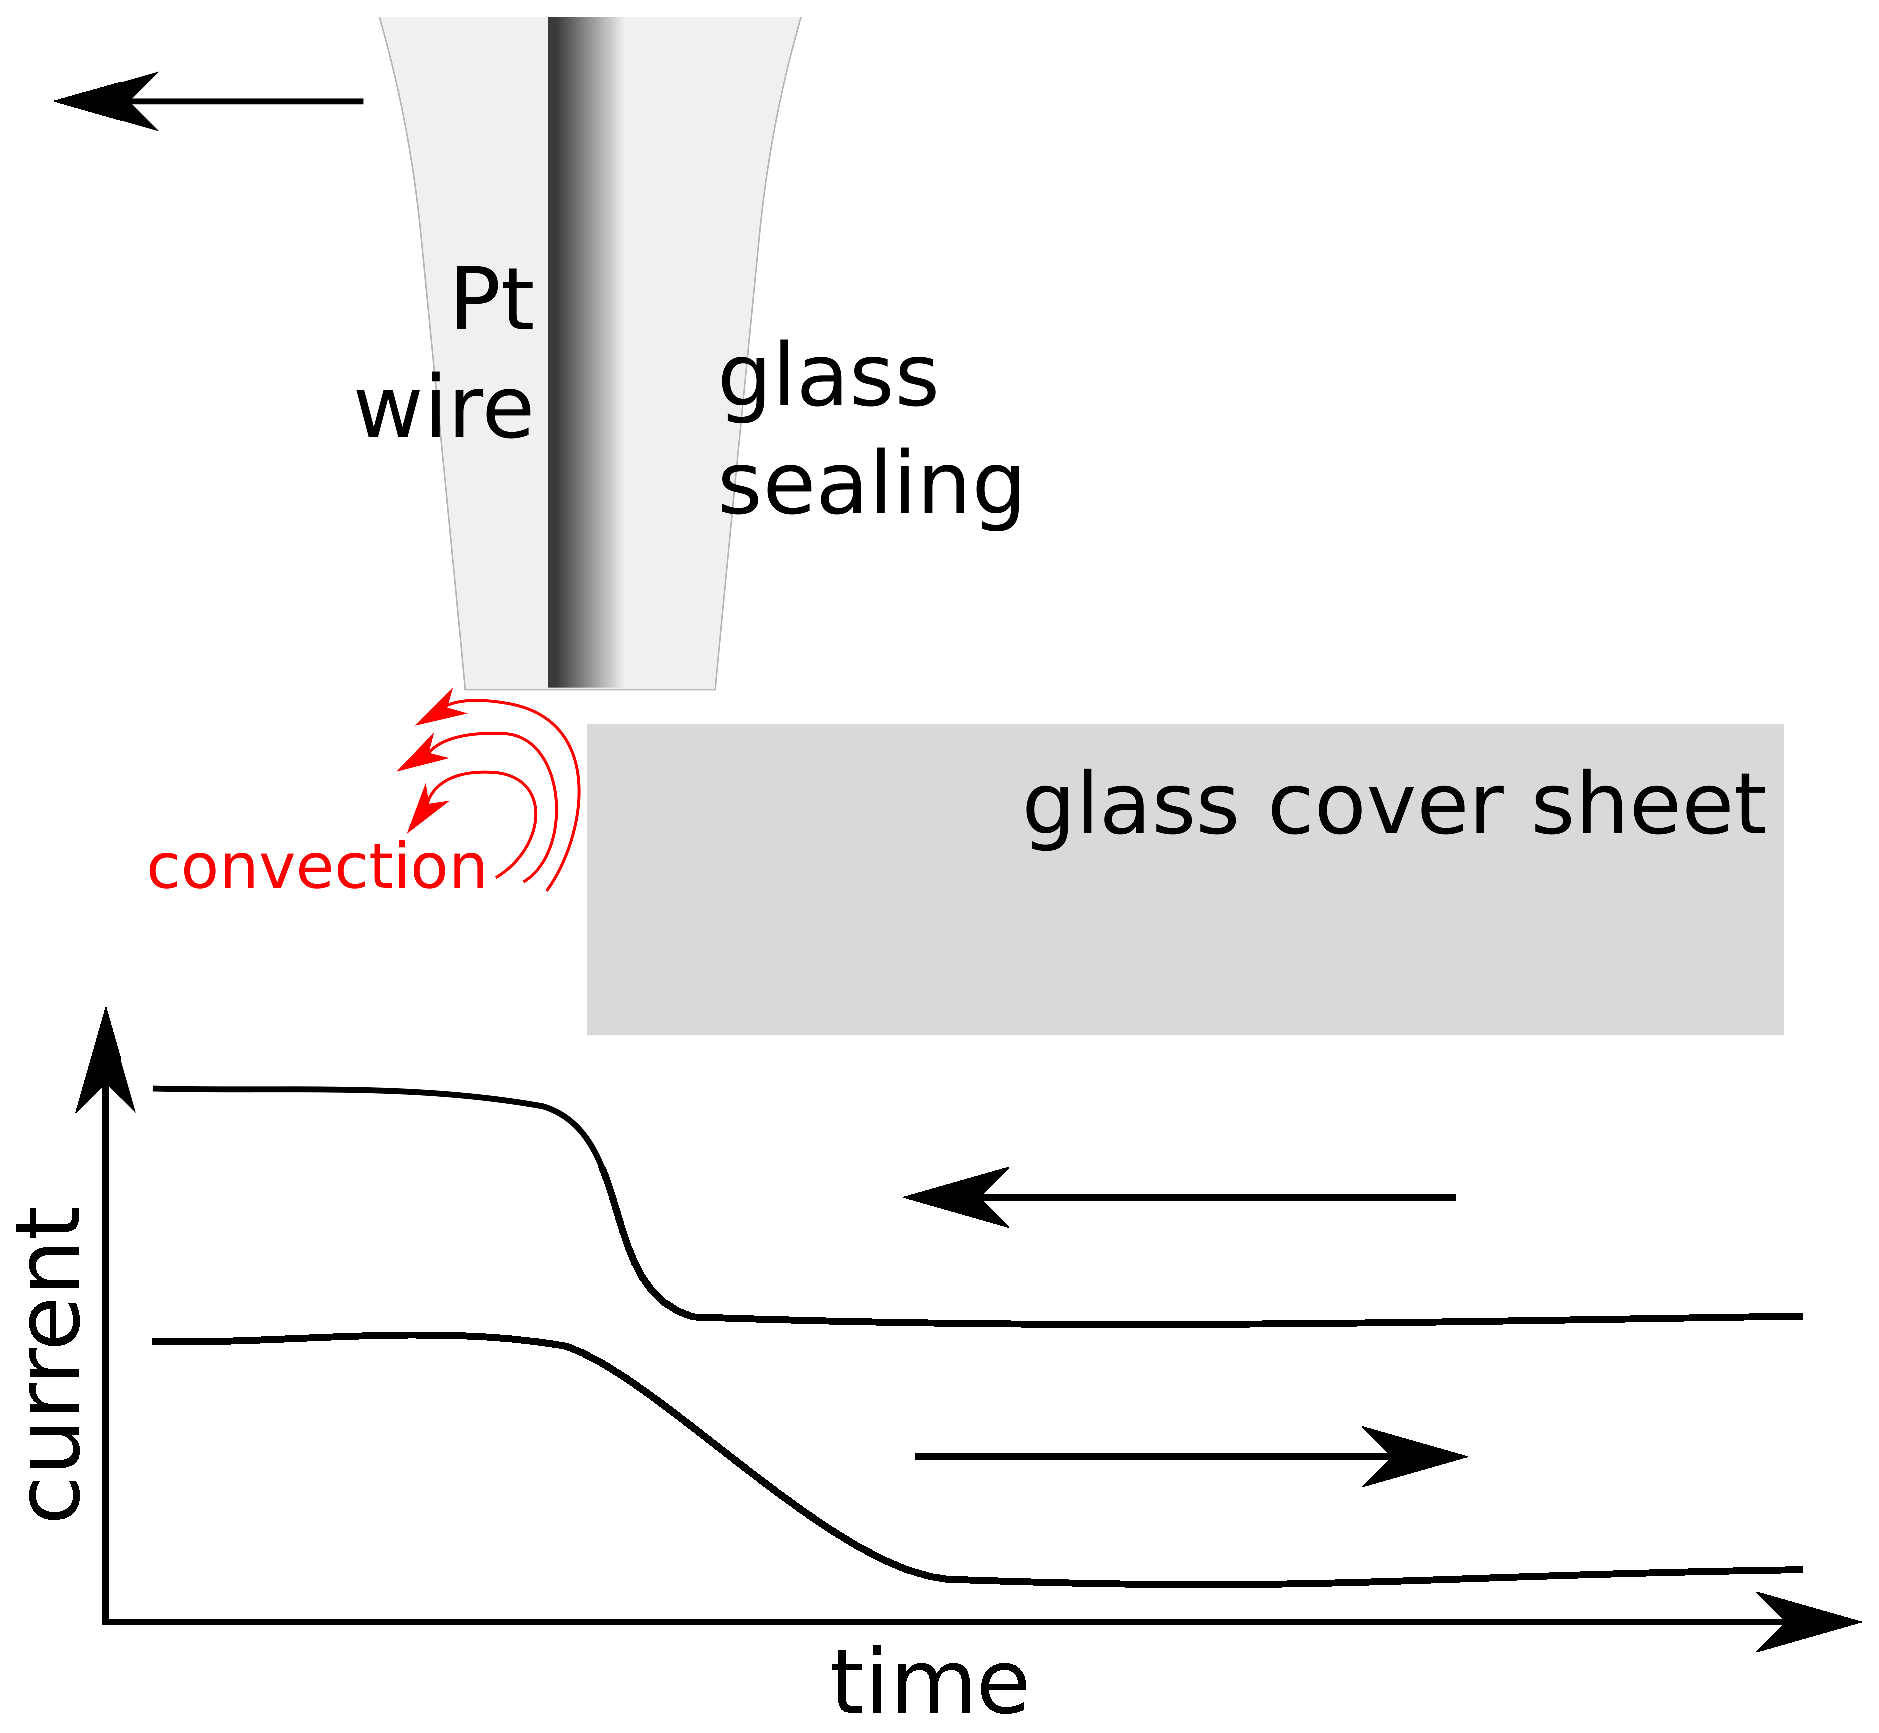
\includegraphics[width=0.3\textwidth]{step_conv.eps}
\caption{The model system to study a simple step function. The oxydation current through the tip is low when the electrode is above the class sheet because of hindered diffusion. The current increases as the tip moves towards the bulk. The transition should be a sharp step function. (A) Sketch of the system. (B) SECM scan result at 5 $\upmu$m/s. (C) SECM scan result at 10 $\upmu$m/s. As it can be seen, the image is a lot more distorted at 10 $\upmu$m/s than at 5 $\upmu$m/s. (D) Attempted deconvolution. The deconvolution in this case did not work, because the raw image was heavily influenced by convection (E). Explanation is in the text.}
\label{fig:step}
\end{figure}

I had to find another model system that acts as a step function. I have built a model that is depicted in Fig. \ref{fig:wire}A. I fixed a d = 10 $\upmu$m Pt wire on the bottom of a Petri--dish. I filled the dish with ferrocenium solution with KCl as background electrolyte. The microphoto of the completed system taken from below can be seen in Fig. \ref{fig:wire}B. Then I approached the wire with the ultramicro-electrode and scanned perpendicularly. Of course this is not an ideal step function, but actually models a cell better. The resulting image is plotted in Fig. \ref{fig:wire}C.


\begin{figure}
\centering
\begin{flushleft}\hspace{3cm}A\end{flushleft}

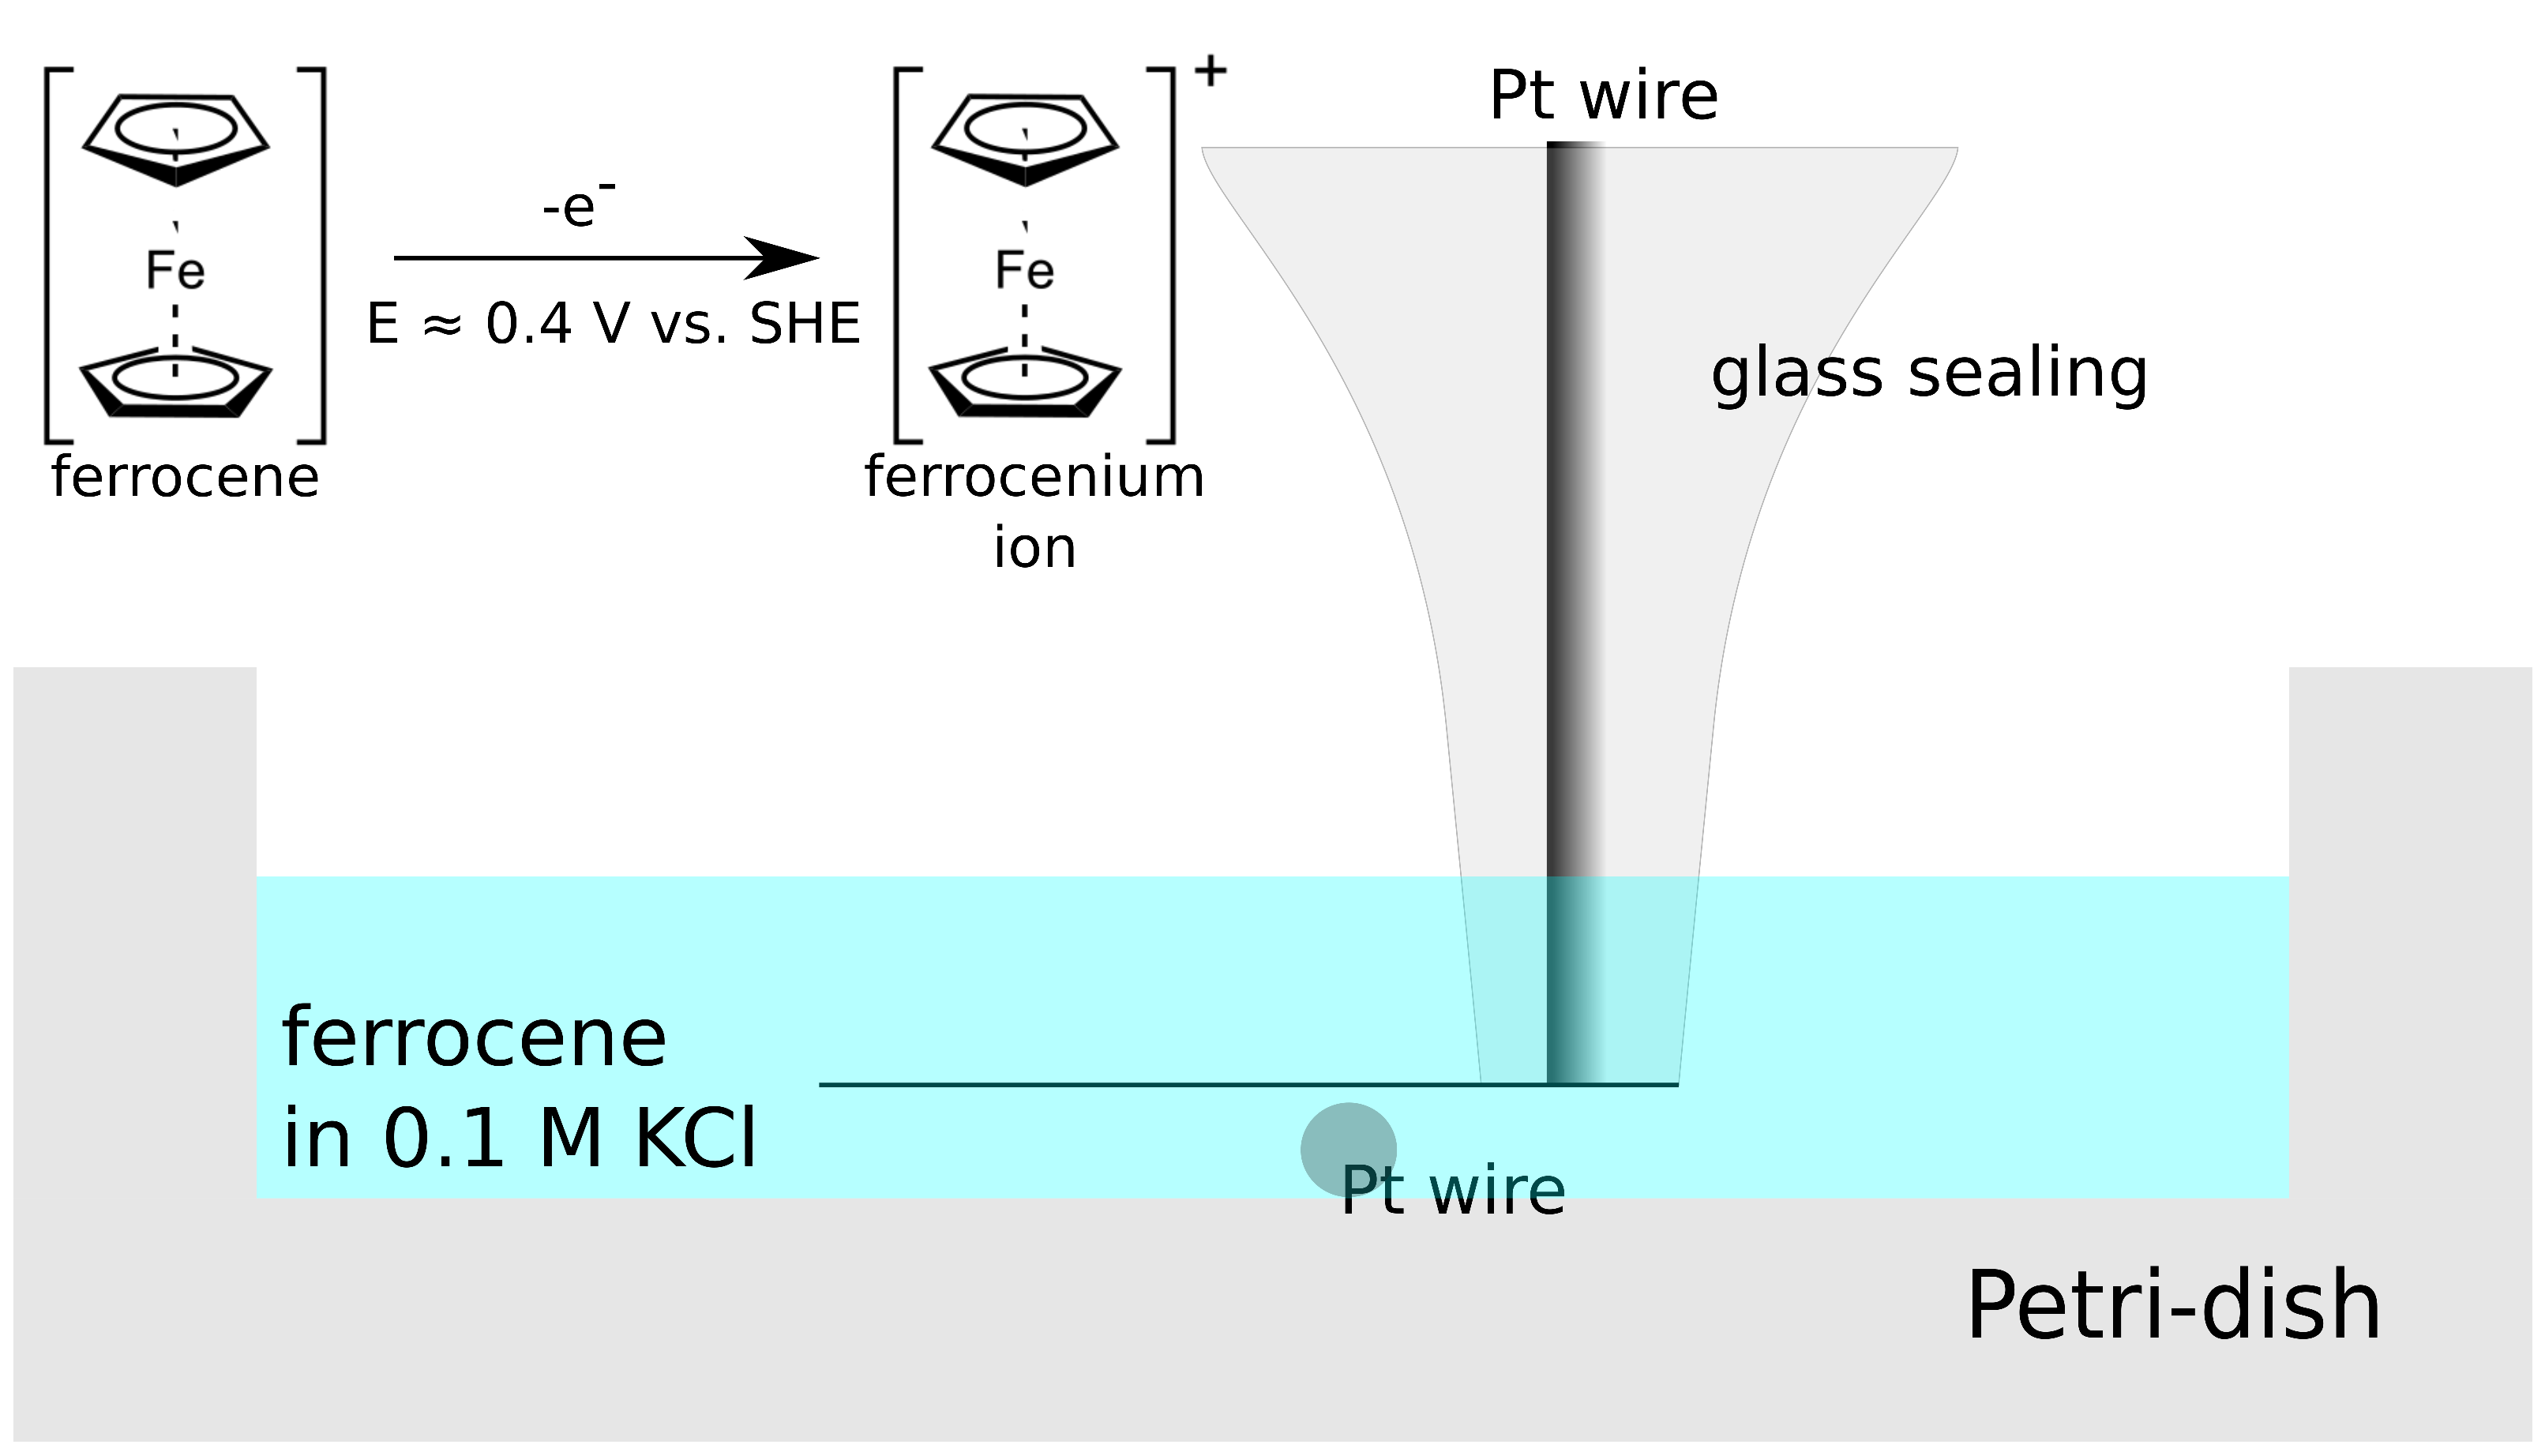
\includegraphics[width=0.5\textwidth]{wire.eps}
\vspace{0.5cm}
\begin{flushleft}\hspace{3cm}B\end{flushleft}

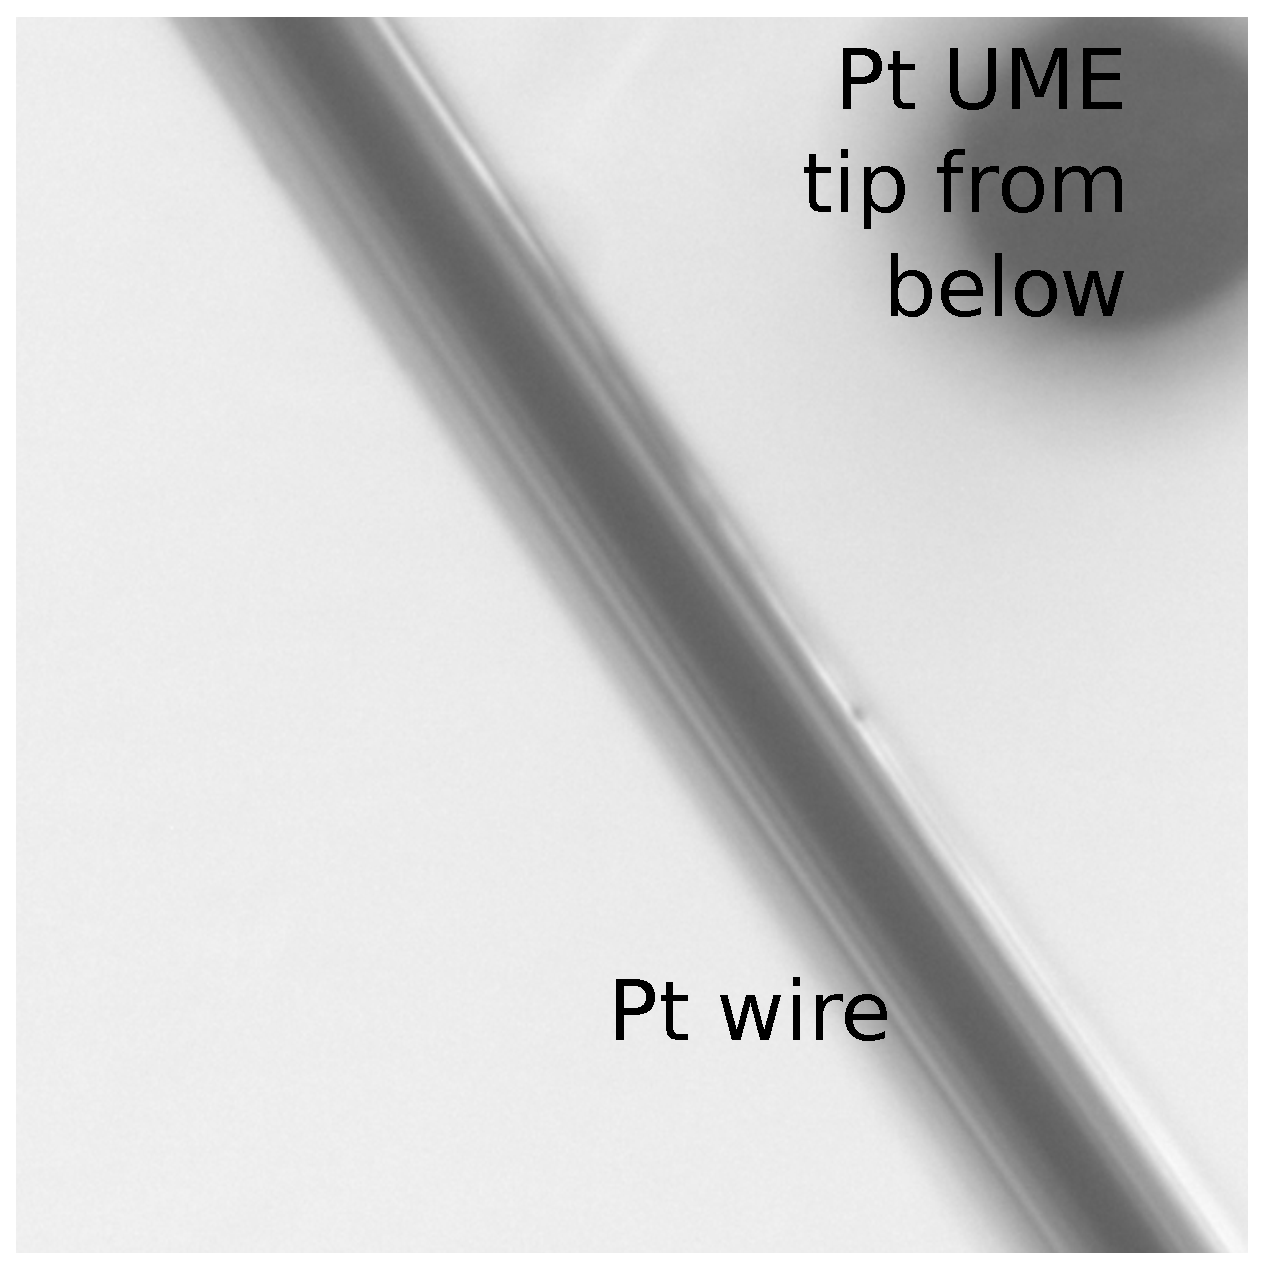
\includegraphics[width=0.3\textwidth]{wire_photo.eps}
\vspace{0.5cm}

\hspace{0cm} C \hspace{5cm} D \hfill

\includegraphics[trim = 10mm 30mm 0mm 20mm, clip, width=0.33\textwidth, angle=-90]{7.eps}\includegraphics[trim = 10mm 30mm 0mm 20mm, clip, width=0.33\textwidth, angle=-90]{7_deconvoluted.eps}
\caption{(A) Sketch of the second model system. In this system I placed a d = 10 $\upmu$m Pt wire on the bottom of a Petri--dish and I scanned above it with a Pt microelectrode. Electrolyte was KCl, electroactive species was ferrocenium. (B) Optical microphoto of the system. (C) Raw image. (D) Deconvoluted image.}
\label{fig:wire}
\end{figure}

The deconvolution on this system worked. The expected shape -- that is a straight stripe across the image -- is restored (Fig. \ref{fig:wire}D). The distortion caused by the long response time of the cell is reduced. The deconvolution function is certainly far from perfect, and the distorion is a lot more complex. The image however improved, and I consider this result a good starting point. 

In the remainder of the report I show the results of the deconvolution of earlier SECM images of immune cells recorded by Dr. Monika Bozem and Phillip Knapp as well as the deconvolution of measurements I have done. This is a big advantage of deconvolution compared to other techniques that aim to reduce distortion: deconvolution can be applied \emph{ex post facto}. I have already shown an example of mapping H$_2$O$_2$ above a monocyte in Fig. \ref{fig:deconv}B. The scanning tip was a 10 $\upmu$m Pt microelectrode. The optical microphoto of the scanned monocyte can be seen in Fig. \ref{fig:deconv}A. The resulting image is distorted (Fig. \ref{fig:deconv}B). After I ran the program above on the dataset plotted in Fig. \ref{fig:deconv}B, the distortion decreased significantly (Fig. \ref{fig:deconv}C). I have managed to successfully deconvolute distorted amperometric SECM images of human immune cells recorded with the HEKA ElProScan SECM system.


The SECM image shown in Fig. \ref{fig:deconv}B was measured with an electrode manufactured by Phillip Knapp, PhD student supervised by Dr. Monika Bozem. I have also constructed my own Pt microelectrodes for further experiments. The so-called \emph{RG}--value is a very important parameter of the amperometric microelectrodes. This is the ratio of the diameter of the whole electrode at the tip (insulation + electroactive part) and the electroactive part. I have managed to create Pt UMEs (ultramicro electrodes) with an RG--value of $\approx$ 2.5. I have used the manufactured electrodes in an interesting application that I have introduced in prof. Hoth's laboratory. Previously H$_2$O$_2$ was measured, because this can be easily done, and it is a good indicator of the general state of a cell undergoing oxidative stress. It is also considered a signalling molecule in the immune system. I've asked Dr. Bozem if it would be interesting to know the concentration of oxygen in the close vicinity of cell. She told me it would be very interesting, so I designed an experiment to demonstarte it. I have mapped the oxygen partial pressure of a human monocyte with the SECM. This can provide information about their metabolic activity. It has great importance in the immune system, where an oxidative burst can significantly influence the O$_2$ concentration nearby the cell. In all cases, oxygen partial pressure is decreasing in the close vicinity of the cell either as a result of cell breathing or increased oxygen uptake to make the oxidative burst possible (Fig. \ref{fig:ox}A).

\begin{figure}
\centering
\begin{flushleft}\hspace{2cm}A\hspace{6cm}B\end{flushleft}
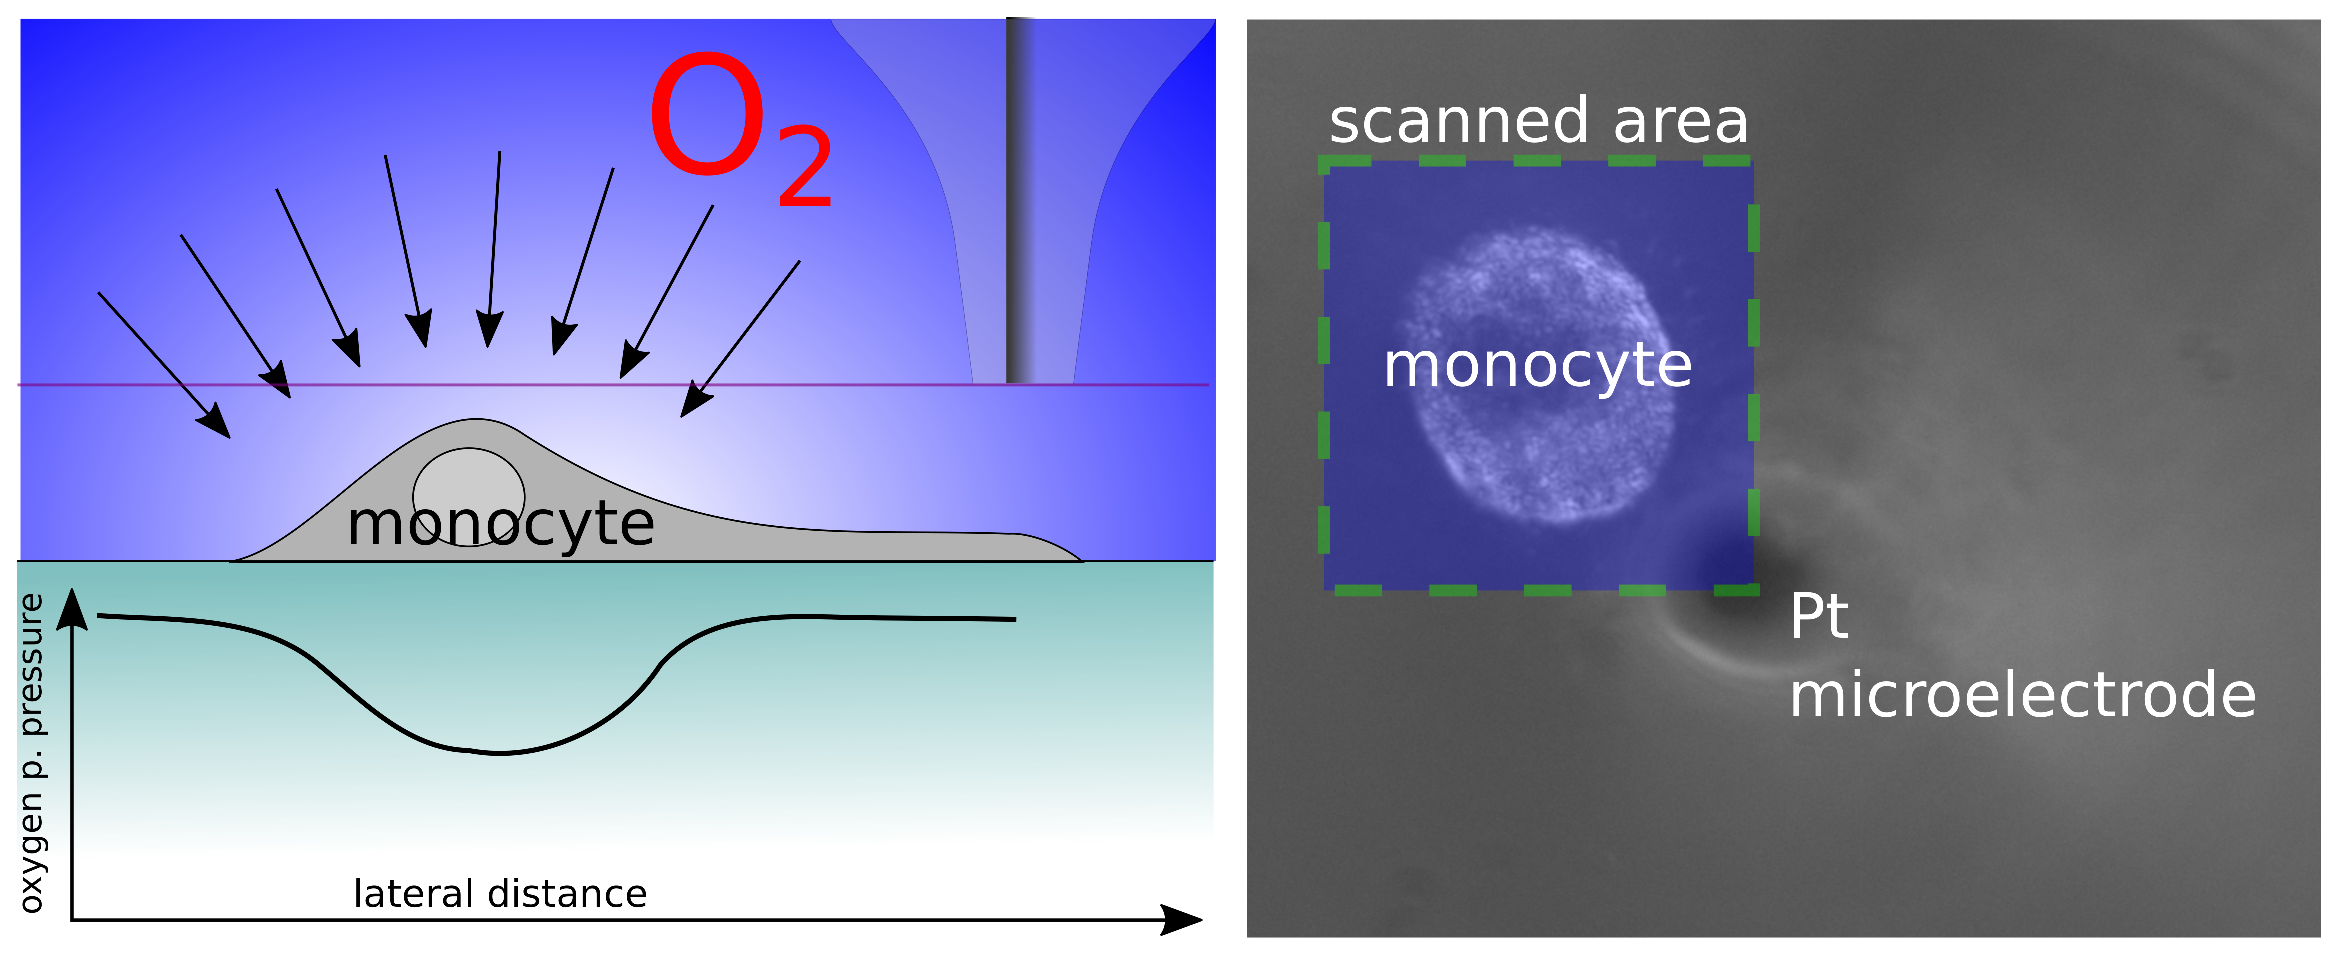
\includegraphics[width=0.8\textwidth]{oxygen.eps}

\vspace{1cm}
\begin{flushleft}\hspace{2cm}C\hspace{7cm}D\end{flushleft}
\includegraphics[trim = 10mm 20mm 0mm 20mm, clip, width=0.4\textwidth, angle=-90]{9_41.eps}\includegraphics[trim = 10mm 20mm 0mm 20mm, clip, width=0.4\textwidth, angle=-90]{9_41_meandered_deconvoluted.eps}

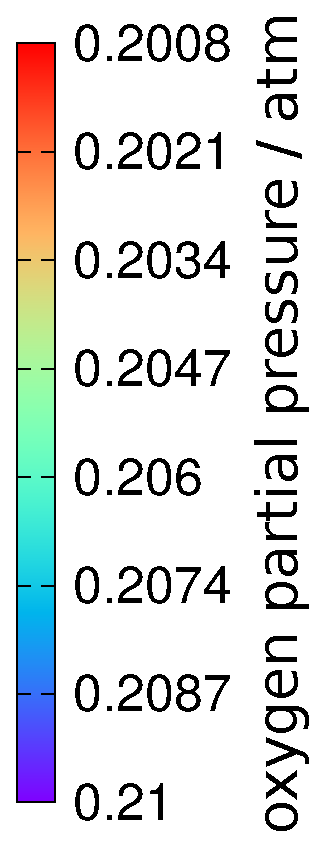
\includegraphics[width=0.15\textwidth, angle=-90]{atm.eps}

\caption{(A) Sketch of the oxygen mapping above the human monocyte. (B) Optical microphoto indicating the monocyte, the scanning tip (10  $\upmu$m Pt) and the scanned area. (C) Raw scan. (D) Deconvoluted image.}
\label{fig:ox}
\end{figure}

I scanned a human monocyte (optical microphoto in Fig. \ref{fig:ox}B) at about 3 $\upmu$m height above the topmost point of the cell. The tip potential was set to -700 mV vs. the Ag/AgCl quasi--reference electrode. At this potential the platinum microelectrode reduces oxygen. The result of the oxygen mapping can be seen in Fig. \ref{fig:ox}C. Once again, the image is distorted. After deconvolution however, the expected image is acquired: a circular shape with a much less distorted contour (Fig. \ref{fig:ox}D). The scanning distortion is almost completely removed in the low concentration region (red), and significantly reduced in the high oxygen concentration region (green-blue). I have calculated the corresponding oxygen partial pressure values based on the linear relationship between the tip current and the oxygen partial pressure. As it can be seen, the decrease is very small, but still very much detectable with this very powerful electroanalytical method.

To summarize this report, I have managed to map hydrogen-peroxyde and oxygen concentration above human immune cells with the SECM. These are two very important species in the immune system, as one is an important signal molecule, and both of them are participating in an oxidative burst. Furthermore, oxygen consumption is a very good indicator of the current metabolic state of a cell. To show that the deconvolution works, I had to reduce the geometry. I have constructed two model systems, and shown that the deconvolution indeed works. 

These are my most important results, and I have included only these as was requested. However, I have done a lot more about several different small topics.  Those results are included in my laboratory notebook. I tried to append it at the end of this report, but even in a heavily compressed form of the combined document exceeded the 5 Mb filesize limit of the DAAD portal upload. I uploaded it separately in a file named ,,notebook\_andras\_kiss.pdf''.

Finally I would like to thank DAAD for making my stay at the University of Saarland possible by providing financial support. The support is greatly appreciated.
\newline

Dr. András Kiss

assistant professor

University of Pécs

Dep. of General and Physical Chemistry

Ifjúság ú. 6

Pécs, 7624

Hungary

tel.: +36 20 388 1324

email: akiss@gamma.ttk.pte.hu

\bibliography{report}{}
\bibliographystyle{plain}


\end{document}
